\documentclass[18pt]{beamer}
%% SLIDE FORMAT
\usepackage[utf8]{inputenc}
\usepackage{algpseudocode}



\title[Programmieren Tutorium]{6. Programmieren Tutorium:\texorpdfstring{\\}{} Objektorientierungs}
\subtitle{Fancy Stuff}
\author{Konstantin Zangerle \texorpdfstring{\\}{} info@konstantinzangerle.de}
\date{7. Dez 2015}

\usepackage{listings}
\usepackage{color}

\definecolor{mygreen}{rgb}{0,0.6,0}
\definecolor{mygray}{rgb}{0.5,0.5,0.5}
\definecolor{mymauve}{rgb}{0.58,0,0.82}

\lstset{ %
  backgroundcolor=\color{white},   % choose the background color
  basicstyle=\footnotesize,        % size of fonts used for the code
  breaklines=true,                 % automatic line breaking only at whitespace
  captionpos=b,                    % sets the caption-position to bottom
  commentstyle=\color{mygreen},    % comment style
  escapeinside={\%*}{*)},          % if you want to add LaTeX within your code
  keywordstyle=\color{blue},       % keyword style
  stringstyle=\color{mymauve},     % string literal style
  showstringspaces=false,
  language=Java
}
\beamersetuncovermixins{\opaqueness<1>{0}}{\opaqueness<2->{0}} %Dont show things after pause 
% Bibliography

\begin{document}

% change the following line to "ngerman" for German style date and logos
%\selectlanguage{ngerman}

%title page
\begin{frame}
\titlepage
\end{frame}

%table of contents
\begin{frame}{Gliederung}
\tableofcontents
\end{frame}

\section{Organsiatorisches}

\begin{frame}{Weihnachten}
 \begin{itemize}
  \item Tutorien bis 22.12
  \item VL am 23.12 fällt aus
  \item 4. Blatt am 9.12 13:00 Ausgabe
  \item Ende 4. Blatt 23.12 13:00
  \item Tuts wieder ab dem 13.1.2016
  \item Dieses Tut also ab dem 18.1.2016
 \end{itemize}

\end{frame}

\section{Listen}
\begin{frame}[fragile]{Code Review}
 \begin{lstlisting}
  static void uneven(int n1, int n2) {
        int n;
        for (int i = n1; i <= n2; i++) {
            
            while ((i % 2) != 0) {
                System.out.print(i + " ");
                break;

            }
        }
    }
 \end{lstlisting}
\end{frame}

\begin{frame}[fragile]{Code Review}
 \begin{lstlisting}
 public static void numbersequence(int lowerBound, int upperBound) {
        int count = lowerBound;

        if (count % 2 == 0) {
            count++;
        }

        if (upperBound % 2 == 0) {
            upperBound -= 1;
        }

        for (; count <= upperBound; count += 2) {
            System.out.print((count != upperBound) ? count + " " : count);
        }

        System.out.println("");
    }


 \end{lstlisting}
\end{frame}


\begin{frame}[fragile]{Code Review}
 \begin{lstlisting}
 if( (number&1) == 0){
            System.out.printf("number %d is even number %n" , number);
        }else{
            System.out.printf("number %d is odd number %n", number);
        }
 \end{lstlisting}
\end{frame}

\subsection{Iterator}
\begin{frame}[fragile]{Iterator}
\begin{lstlisting}
 List<String> list = new ArrayList<String>();
list.add("Ente");
list.add("Schinken");
list.add("Truthahn");
 
for(String name: list) System.out.println(name);
\end{lstlisting}
 
\end{frame}




\section{Vererbung}
\subsection{Einführung}
\begin{frame}{Vererbung}

 \begin{itemize}
 \item Ein PKW ist ein Fahrzeug, ein Zweirad ist ein Fahrzeug, 
  \item Eine Limousine ist ein Fahrzeug, aber nicht jedes Fahrzeug ist eine Limousine
  \item Jedes Cabrio kann das Dach öffnen bzw. schließen, bei PKWs macht das (meistens) keinen Sinn.
 \end{itemize}
\end{frame}

\begin{frame}{Genauer: Vererbung}
 \begin{itemize}
  \item Vererbung ist eine ``ist''-Beziehung
  \item Alle Eigenschaften (Attribute) werden übernommen!
  \item Alle Methoden werden übernommen.
  \item Kinder haben aber auch Freiheiten diese zu ändern!
 \end{itemize}
\end{frame}



\section{Methoden und Methoden in Vererbung}
\begin{frame}[fragile]{Überschreibung von Methoden}
Betrachte die Klassen
\begin{lstlisting}
public class Motor {
  public void starten() { ... }
}

public class DieselMotor extends Motor {
  @Override
  public void starten() { ... }
} 
\end{lstlisting}
\end{frame}



\begin{frame}{Konstruktoren und super}
 \begin{alertblock}{Ein wichtiger Unterschied}
  In Konstruktoren muss der super() Konstruktor als erstes aufgerufen werden,
  oder gar nicht!
 \end{alertblock}
\end{frame}


\begin{frame}[fragile]{Generische Klassen}
 \begin{lstlisting}
  ArrayList<String> liste = new ArrayList<String>(); //oder...
  Liste liste = new ArrayList<String>();
 \end{lstlisting}
\end{frame}


\begin{frame}[fragile]{Schnittstellen}
\begin{lstlisting}
 interface Motor {
  public void starten();
  public int getLeistung();
 }
 \end{lstlisting}
 \begin{itemize}
  \item Interfaces stellen eine Schablone dar.
  \item Interfaces geben die Gewissheit, das Klassen, die diese implementieren, Funktionen besitzen.
  \item Interfaces haben keine Attribute.
 \end{itemize}

\end{frame}

\begin{frame}[fragile]{Javadoc}
 Javadoc sind Kommentare mit folgendem Schema:
 \begin{lstlisting}
  /**
 * Kurzbeschreibung der Funktionalitaet in einem Satz.
 * Weitere Details folgen darauf.
 * 
 * Beschreibung von Parametern, Rueckgabewerten und co.
 * geschieht durch spezielle Tags.
 */
 \end{lstlisting}
Außerdem können ``Tags'' verwendet werden, bspw. @author, @version, @param, @return, @throws
Siehe dazu den Eintrag im Programmieren Wiki
\scriptsize
\verb|https://ilias.studium.kit.edu/goto.php?target=wiki_349162_Javadoc|
\end{frame}




\subsection{Java-Object}
\begin{frame}{Java: Object}
  \small
 Jedes Objekt hat folgende Methoden:
 \begin{itemize}
  \item clone()
  \item equals(Object obj)
  \item finalize()
  \item getClass()
  \item hashCode()
  \item notify()
  \item notifyAll()
  \item toString()
  \item wait()
  \item wait(long timeout)
  \item wait(long timeout, int nanos)
 \end{itemize}
 Aber warum? \\
 \large Antwort: Vererbung
 

\end{frame}

\begin{frame}[fragile]{Abstrakte Klassen}
 Abstrakte Klassen sind Klassen, die nicht direkt instanziert werden können.
 \begin{lstlisting}
    public abstract class AbstracterSchinken {
      public String name;
    }
 \end{lstlisting} 
 Natürlich gilt das auch für Methoden
 \begin{lstlisting}
    public abstract class AbstrakterSchinken {
      public abstract void Abschneiden();
    }
 \end{lstlisting} 
Was ist der Unterschied einer abstrakten Klasse zu ``Interfaces``?
\end{frame}

\begin{frame}[fragile]{Inhaltliche Gleichheit}
 Java erlaubt es zunächst auf Identität zu überprüfen.
 Mittels \verb|==|
 \begin{itemize}
  \item Das funktioniert nicht bei Strings.
  \item Zumindest meistens.
 \end{itemize}
\end{frame}
\begin{frame}[fragile]{Prüfen auf ''Inhaltliche Gleichheit''}
 Mittels überschreiben der \verb|equals|-Methode. Alles klar? 
 Was gibt es zu beachten?:
 Equals muss erfüllen
 \begin{enumerate}
  \item Reflexiv
  \item Symmetrisch
  \item Transitiv
  \item Konsistenz
  \item für x nicht null gibt x.equals(null) false
 \end{enumerate}
\end{frame}

\begin{frame}[fragile]{Beispiel}
 \begin{lstlisting}
  public boolean equals(Object other) {
   if (this == other)
      return true;
   if (other == null)
      return false;
   if (other.getClass() != getClass())
      return false;

   if (!(s.equals(((MyClass)other).s)))
      return false;
   if (i != ((MyClass)other).i)
      return false;
   ...
   return true;
   } 
 \end{lstlisting}
\end{frame}

\begin{frame}{Final}
``Bis hierher darfst du und nicht weiter, hier muss sich legen deiner Wogen Stolz''. (Ijob 38,11)
  \pause
  
  \begin{itemize}
   \item Klassen: Kann nicht abgeleitet werden
   \item Methoden: Kann nicht überschrieben/versteckt werden
   \item Variablen: Kann nur einmal initialisiert werden, jede Änderung erzeugt einen Fehler
  \end{itemize}
\end{frame}

\begin{frame}[fragile]{Verkettete Listen und Iteratoren}
\begin{lstlisting}[language=java]
    public static void main(String[] args) {
        TreeSet<String> set = new TreeSet<String>();
        for (int i = 0; i < 20; i++) {
            set.add(new Integer(i).toString());
        }
        for (Iterator<String> it = set.iterator(); it.hasNext();) {
            String s = it.next();
            if (s.equals("15"))
                it.remove();
            System.out.println(s); // "15" noch enthalten
        }
        Iterator<String> iter = set.iterator();
        while (iter.hasNext()) {
            String s = iter.next();
            // if(s.equals("15")) set.remove(s); // ConcurrentModificationException
            iter.remove();
            System.out.println(s); // "15" entfernt
        }
    }
\end{lstlisting}

\end{frame}


\begin{frame}{Queue, Stack, Priority Queue}
\begin{itemize}
 \item Priority Queue \url{http://stackoverflow.com/questions/683041/java-how-do-i-use-a-priorityqueue}
 \item Stack \url{http://www.java-tutorial.org/stack.html}
\end{itemize}

 
\end{frame}

\begin{frame}[fragile]{instanceof}
 \begin{lstlisting}
class Parent {  }
class Child extends Parent {   }

public class Main {
  public static void main(String[] args) {

    Child child = new Child();
    if (child instanceof Parent) {
      System.out.println("passt");
    }

  }

}
 \end{lstlisting}

\end{frame}


%Lacher zum Schluss
\begin{frame}
 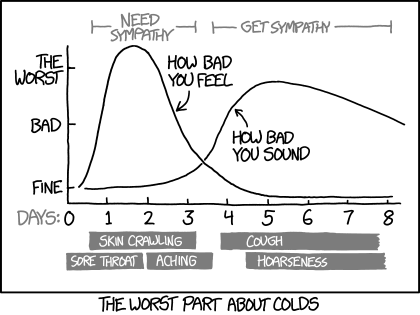
\includegraphics[scale=0.7]{colds}
 
 \tiny{Quelle: xkcd.com/1612}
\end{frame}


\end{document}
%%%%%%%%%%%%%%%%%%%%%%%%%
%Bausteine
%nice to have code
%%%%%%%%%%%%%%%%%%%%%%%%%%



%%%%% Bausteine Folie mit Java-Code
%\begin{frame}[fragile]{bla}
%\begin{exampleblock}{bla}
%\begin{lstlisting}[language=java]
%\end{lstlisting}
%\end{exampleblock}
%\end{frame}
